% Paginação de uma face: margens e cabeçalhos fixos em todas as páginas.
\documentclass[a4paper,11pt,oneside,openany]{book}

\usepackage{amsmath}
% Permite a hifenização das palavras acentuadas do conteúdo em português.
\usepackage[T1]{fontenc}
% Mantém fontes escaláveis da família Computer Modern com a codificação T1.
\usepackage{lmodern}
\usepackage[utf8]{inputenc}
\usepackage[portuguese]{babel}
\usepackage{graphicx}
\usepackage{pdfpages}
\usepackage{xcolor}
% Bloco de texto centrado, com espaço para diagramas legíveis.
\usepackage[a4paper,left=27.5mm,right=27.5mm,top=25mm,bottom=25mm,
    includeheadfoot,headheight=16pt,headsep=5mm,footskip=10mm]{geometry}
\usepackage{fancyhdr}
\usepackage{setspace}
\usepackage{array}
\usepackage{colortbl}
%\usepackage{multirow}
\usepackage{amssymb}
\usepackage{lscape}
% Suporte às citações de texto, tabelas e endereços do conteúdo migrado.
\usepackage{csquotes}
\usepackage{booktabs}
\usepackage{tabularx}
% Tabelas de rastreabilidade e características com continuação entre páginas.
\usepackage{longtable}
% Compatibilidade com versões de longtable anteriores à correção de 2026:
% usar encolhimento finito nas quebras de página, em vez de \vss.
% https://github.com/latex3/latex2e/issues/1907
\usepackage{etoolbox}
\makeatletter
\patchcmd{\LT@output}{\vss}{\vskip\z@ plus\maxdimen minus\normalbaselineskip}{}{}
\patchcmd{\LT@output}{\vss}{\vskip\z@ plus\maxdimen minus\normalbaselineskip}{}{}
\makeatother
\usepackage{xurl}
\usepackage{acronym}
\newcommand{\acroemph}[1]{\textit{#1}}
% Diagramas vetoriais: estilos comuns, legíveis também em escala de cinzentos.
\usepackage{tikz}
\usetikzlibrary{arrows.meta,positioning,calc,fit,backgrounds}
\definecolor{LasetBlue}{HTML}{234D65}
\definecolor{LasetTeal}{HTML}{287D83}
\definecolor{LasetTint}{HTML}{EDF3F6}
\definecolor{LasetGrey}{HTML}{555E64}
\tikzset{
    bloco/.style={draw=LasetBlue,fill=LasetTint,rounded corners=2pt,
        line width=0.7pt,align=center,inner sep=5pt,
        font=\sffamily\small,text=black},
    nucleo/.style={bloco,fill=LasetBlue,text=white},
    auxiliar/.style={bloco,draw=LasetGrey,fill=black!3},
    opcional/.style={auxiliar,dashed},
    fluxo/.style={-{Latex[length=2.2mm,width=1.5mm]},
        draw=LasetBlue,line width=0.85pt},
    duplo/.style={{Latex[length=2mm,width=1.4mm]}-{Latex[length=2mm,width=1.4mm]},
        draw=LasetBlue,line width=0.85pt},
    ligacao/.style={draw=LasetBlue,line width=0.8pt},
    legenda/.style={font=\sffamily\footnotesize,align=center,text=LasetGrey},
    mini/.style={bloco,font=\sffamily\footnotesize,inner sep=3pt}
}
\newcommand{\Diagrama}[1]{%
    \begingroup\setstretch{1}\hyphenpenalty=10000\exhyphenpenalty=10000%
    \input{./Figuras/diagramas/#1.tex}\endgroup}

%\usepackage{subfigure}
\setlength{\unitlength}{1mm}
\renewcommand{\baselinestretch}{1.5}
\clubpenalty=10000
\widowpenalty=10000
\displaywidowpenalty=10000
\newif\ifRequisitos
\newif\ifProjecto
\newif\ifFinal

\Requisitostrue
\Projectotrue
\Finalfalse
 
\newcommand{\Author}{Francisco Liquito\\ Pedro Ribeiro}
\newcommand{\Title}{Sistema de Escrita/Leitura Multi-Protocolo\\
(I2C, RS232, RS485, CAN FD, Ethernet, PWM e GPS)}
% Data da entrega: atualizar à mão em cada fase (não usar \today).
\newcommand{\DataRelatorio}{novembro de 2026}
% TODO: confirmar os nomes dos docentes; não estão identificados no projeto.

\begin{document}
	\begin{titlepage}
		%---------------------------------------------
%   Capa do Relatório
%---------------------------------------------
\begingroup
\setstretch{1}
\thispagestyle{empty}
\centering
% A largura da capa é centrada na página, sem deslocamentos absolutos.
\noindent\makebox[\textwidth][c]{%
    \begin{minipage}[t][0.96\textheight][s]{150mm}
        \centering
        {\huge\textsc{Laboratório de Sistemas Autónomos}\par}
        \vspace{15mm}
        
\includegraphics[height=20mm]{./Figuras/logo_ISEP.jpg}\par
        \vspace{5mm}
        
\includegraphics[height=15mm]{./Figuras/logo_LSA.jpg}\hspace{3mm}%
        
\includegraphics[height=15mm]{./Figuras/inesc.jpg}\par
        \vfill
        \ifFinal
            {\LARGE Relatório Final\par}
        \else
            \ifProjecto
                {\Large Relatório de Projecto\par}
            \else
                \ifRequisitos
                    {\Large Relatório de Análise de Requisitos\par}
                \else
                    {\Large\textcolor{red}{Não foi definido o tipo de relatório}\par}
                \fi
            \fi
        \fi
        \vspace{8mm}
        {\LARGE\Title\par}
        \vfill
        {\large\Author\par}
        \vfill
        {\large Mestrado de Sistemas Autónomos\par}
        \vspace{2mm}
        {\large LaSET - Laboratório de Sistemas Embebidos e Tecnologias\par}
        \vspace{4mm}
        {\large\DataRelatorio\par}
    \end{minipage}%
}
\par
\endgroup

	\end{titlepage}
	\pagestyle{plain}
	\pagenumbering{roman}
	\tableofcontents
	\listoffigures
	\listoftables
	% Lista de acrónimos (pacote acronym).
\chapter*{Lista de Acrónimos}
\addcontentsline{toc}{chapter}{Lista de Acrónimos}
\begin{acronym}[RNF]
  \acro{CAN}{\acroemph{Controller Area Network}}
  \acro{CANFD}[CAN FD]{\acroemph{CAN with Flexible Data-Rate}}
  \acro{CRC}{\acroemph{Cyclic Redundancy Check}}
  \acro{DP}{Decisão de Projeto}
  \acro{ESD}{\acroemph{Electrostatic Discharge}}
  \acro{FCS}{\acroemph{Frame Check Sequence}}
  \acro{GPS}{\acroemph{Global Positioning System}}
  \acro{GUM}{\acroemph{Guide to the Expression of Uncertainty in Measurement}}
  \acro{I2C}{\acroemph{Inter-Integrated Circuit}}
  \acro{IP}{\acroemph{Internet Protocol}}
  \acro{MAC}{\acroemph{Media Access Control}}
  \acro{MCU}{\acroemph{Microcontroller Unit}}
  \acro{MPU}{\acroemph{Microprocessor Unit}}
  \acro{ND}{Não determinado}
  \acro{NS}{Não especificado}
  \acro{NTP}{\acroemph{Network Time Protocol}}
  \acro{P}{Problema ou necessidade (P01--P04)}
  \acro{PC}{Computador pessoal}
  \acro{PCB}{\acroemph{Printed Circuit Board}}
  \acro{PHY}{Camada física (\acroemph{Physical Layer})}
  \acro{PoE}{\acroemph{Power over Ethernet}}
  \acro{PPS}{\acroemph{Pulse Per Second}}
  \acro{PWM}{\acroemph{Pulse Width Modulation}}
  \acro{RAM}{\acroemph{Random Access Memory}}
  \acro{RF}{Requisito Funcional}
  \acro{RNF}{Requisito Não Funcional}
  \acro{RS232}{\acroemph{Recommended Standard 232}}
  \acro{RS485}{\acroemph{Recommended Standard 485}}
  \acro{RTOS}{\acroemph{Real-Time Operating System}}
  \acro{SDA}{\acroemph{Serial Data}}
  \acro{SCL}{\acroemph{Serial Clock}}
  \acro{SO}{Sistema Operativo}
  \acro{SPI}{\acroemph{Serial Peripheral Interface}}
  \acro{TCP}{\acroemph{Transmission Control Protocol}}
  \acro{UC}{Caso de Utilização (\acroemph{Use Case})}
  \acro{UDP}{\acroemph{User Datagram Protocol}}
\end{acronym}


	\mainmatter
	\setlength{\headsep}{5mm}
	\setlength{\headheight}{16pt}
	\pagestyle{fancy}
	\fancyhf{}
	\fancyhead[L]{\small\itshape\nouppercase{\leftmark}}
	\fancyhead[R]{\small\itshape\nouppercase{\rightmark}}
	\fancyfoot[C]{\thepage}
	\raggedbottom

	\renewcommand{\sectionmark}[1]{\markright{\arabic{chapter}.\arabic{section}. #1}}
	\renewcommand{\chaptermark}[1]{\markboth{Capítulo \arabic{chapter} }{}}

	\pagenumbering{arabic}
	\ifRequisitos
	%-----------------------------------------------------------
%   Capítulo 1 - Introdução
%-----------------------------------------------------------
\chapter{Introdução}
\label{cap:introducao}

\section{Enquadramento e Motivação}

O projeto de um sistema de leitura e escrita multiprotocolo insere-se
no contexto dos sistemas embebidos e autónomos em que coexistem diferentes
tecnologias de comunicação. O trabalho abrange I2C, RS232, RS485, CAN e
Ethernet e é apresentado neste relatório numa fase preliminar de definição,
centrada no enquadramento do problema e na organização do estudo e do
desenvolvimento.

Os sistemas autónomos e os sistemas embebidos integram funções de
perceção, processamento, controlo e atuação que dependem da troca de
informação entre os seus elementos. A aquisição de dados de sensores,
o envio de comandos a atuadores e a comunicação com controladores ou
equipamentos de supervisão podem envolver tecnologias de comunicação
distintas numa mesma instalação. Esta coexistência resulta das
características dos dispositivos e das funções que desempenham, bem
como da necessidade de integrar equipamentos desenvolvidos em momentos
ou contextos diferentes.

Neste contexto, sensores, atuadores, controladores e outros equipamentos
podem disponibilizar interfaces como I2C, RS232, RS485, CAN e Ethernet.
Estas tecnologias apresentam diferenças nas características elétricas,
na organização das ligações e nos mecanismos de comunicação que
suportam. Por conseguinte, a ligação de um novo equipamento exige a
análise da compatibilidade da interface e da forma como os dados são
transmitidos e recebidos, além da compreensão do seu significado para
a aplicação.

O problema central reside na heterogeneidade destas interfaces e na
dificuldade de integrar operações de leitura e escrita sobre equipamentos
com formas de acesso distintas. O suporte de cada tecnologia pode exigir
configurações, procedimentos de comunicação e mecanismos de tratamento
de erros específicos. Quando estas particularidades são tratadas de
forma dispersa na aplicação, a inclusão ou substituição de equipamentos
pode implicar alterações em várias partes do sistema, dificultando a
manutenção e a reutilização das funções de comunicação. Além disso, a
disponibilidade de uma ligação compatível não assegura, por si só, a
interpretação correta dos dados trocados.

A relevância do trabalho reside, assim, na possibilidade de organizar de
forma coerente os mecanismos de acesso aos equipamentos, facilitando a
integração e a evolução de sistemas com diferentes tecnologias de
comunicação.

\section{Cenários de aplicação}

\textit{TODO: definir os cenários de aplicação após validação do âmbito do projeto.}

\section{Objectivos}

\subsection{Objetivo Geral}

Estudar e desenvolver um sistema capaz de realizar operações de leitura
e escrita através das tecnologias de comunicação I2C, RS232, RS485,
CAN e Ethernet.

\subsection{Objetivos Específicos}

Para concretizar o objetivo geral, estabelecem-se os seguintes objetivos
específicos:

\begin{enumerate}
    \item Estudar as características de I2C, RS232, RS485, CAN e Ethernet
    relevantes para a realização de operações de comunicação.

    \item Analisar as diferenças e limitações das cinco tecnologias,
    identificando as suas implicações para a integração num mesmo sistema.

    \item Definir uma arquitetura de integração das cinco interfaces,
    identificando os blocos funcionais e as respetivas ligações.

    \item Implementar as funções de comunicação necessárias à transmissão
    e receção de dados através de cada uma das cinco interfaces.

    \item Validar experimentalmente as operações de transmissão e receção
    em cada interface, de acordo com os requisitos que venham a ser
    consolidados.
\end{enumerate}

\section{Estrutura do Relatório}

O Capítulo~\ref{cap:introducao} apresenta o enquadramento, a motivação
e os objetivos do trabalho. O Capítulo~\ref{cap:estado-arte} organiza
o Estado da Arte sobre as tecnologias abrangidas.
O Capítulo~\ref{cap:requisitos} distingue as capacidades previstas,
as propostas preliminares e as questões a esclarecer com os docentes.
Por fim, o Capítulo~\ref{cap:arquitectura} apresenta os blocos funcionais
abstratos da Arquitetura de Alto Nível, cuja concretização depende
do estudo e da consolidação dos requisitos.

	%-----------------------------------------------------------
%   Capítulo 2 - Estado da Arte 
%-----------------------------------------------------------
\chapter{Estado da Arte}
\label{cap:estado-arte}

\section{Comunicação em Sistemas Embebidos e Autónomos}

Nos sistemas embebidos e autónomos, as interfaces de comunicação respondem
a diferentes escalas de interligação e requisitos de funcionamento. O I2C
é utilizado na comunicação entre circuitos e periféricos, enquanto
interfaces como RS485 permitem interligar equipamentos em aplicações de
automação industrial e de
edifícios~\cite{nxp_um10204_2021,stiller_rs485_2015}.

Neste contexto, importa distinguir a camada física, relativa à transmissão
de sinais no meio, da camada de ligação de dados, que organiza a
transferência de tramas e o acesso ao meio. O protocolo de aplicação
define as operações e o significado dos dados trocados. A existência de
interfaces elétricas compatíveis não garante compatibilidade nas camadas
superiores~\cite{dodson_rs232_2023,stiller_rs485_2015,ieee_8023_2018}.

Estas tecnologias não ocupam todas o mesmo âmbito na comunicação.
Enquanto o I2C inclui regras próprias de transferência no barramento,
RS232 e RS485 caracterizam sobretudo a interface física. Modbus RTU
constitui um exemplo de protocolo que pode operar sobre ligações série,
sem ser uma propriedade intrínseca dessas
interfaces~\cite{nxp_um10204_2021,modbus_serial_2006}.

\section{I2C}

O I2C utiliza um barramento série síncrono partilhado constituído por duas
linhas: SDA, destinada à transferência de dados, e SCL, utilizada para o
sinal de relógio. Nos modos \textit{Standard-mode}, \textit{Fast-mode} e
\textit{Fast-mode Plus}, a sinalização baseia-se tipicamente em saídas de dreno ou
coletor aberto e na polarização das linhas por
\textit{pull-up}~\cite[sec.~3.1]{nxp_um10204_2021}.

Nestes modos, um controlador inicia cada transferência e gera o relógio;
o dispositivo alvo é selecionado por endereço de 7 ou 10 bits. Os dados circulam em bytes,
com indicação de confirmação ou não confirmação (ACK/NACK). A comunicação
é bidirecional, existindo arbitragem quando vários controladores disputam
o barramento~\cite[secs.~3.1.5--3.1.11]{nxp_um10204_2021}.

O reduzido número de linhas e o endereçamento integrado favorecem a
ligação local de periféricos, como sensores, memórias e expansores de
entradas e saídas, habitualmente no mesmo equipamento. Este contexto de
interligação entre circuitos distingue-se das redes distribuídas com
CAN ou RS485. A capacidade de expansão e a velocidade ficam condicionadas
pela capacitância do barramento e pelos tempos de subida dos
sinais~\cite[secs.~2 e~7]{nxp_um10204_2021}.

\section{RS232}

A interface RS232 estabelece ligações série ponto a ponto, com sinalização
não diferencial referida a uma massa comum. Os estados lógicos são
representados por tensões de polaridade positiva ou negativa; as linhas
distintas de transmissão e receção permitem comunicação simultânea nos
dois sentidos (\textit{full-duplex})~\cite[secs.~2.1 e~2.2]{dodson_rs232_2023}.

A norma define aspetos elétricos, funcionais e mecânicos. As designações
DTE (\textit{Data Terminal Equipment}) e DCE (\textit{Data Communication
Equipment}) distinguem funções dos equipamentos; deste âmbito não resulta
um mecanismo de endereçamento multiponto nem um protocolo de
aplicação~\cite[sec.~2]{dodson_rs232_2023}.
É frequente a utilização de comunicação assíncrona, mas a norma também
contempla sinais de temporização~\cite{ti_rs232_2002,dodson_rs232_2023}.

A RS232 permite uma ligação ponto a ponto simples e tem sido amplamente
utilizada na interligação de periféricos, modems e equipamentos de teste.
As principais limitações incluem a suscetibilidade ao ruído e as restrições de alcance e débito;
o comprimento admissível depende das características elétricas da
ligação, em particular da sua
capacitância~\cite{ti_rs232_2002,dodson_rs232_2023}.

\section{RS485}

RS485 define as características elétricas de emissores e recetores para
comunicação série diferencial multiponto. A informação é representada
pela diferença de tensão entre dois condutores, e vários nós podem
partilhar o barramento~\cite{stiller_rs485_2015,ti_rs485_an1057_2013}.

Na configuração \textit{half-duplex}, um par de sinais permite transmissão
alternada nos dois sentidos; a configuração \textit{full-duplex} utiliza
dois pares. A documentação recomenda uma disposição linear, com
derivações curtas, para reduzir problemas de
propagação~\cite[secs.~2 e~3]{ti_rs485_an1057_2013}.

A norma não define o protocolo de aplicação. Por conseguinte, o
endereçamento e a coordenação do acesso ao meio têm de ser tratados
acima da camada elétrica; a transmissão simultânea de vários emissores
no mesmo par pode causar contenção~\cite[secs.~1 e~10]{ti_rs485_an1057_2013}.

A robustez a ruído proporcionada pela sinalização diferencial e o suporte
multiponto constituem vantagens em aplicações de automação industrial,
automação de edifícios e controlo de motores~\cite{stiller_rs485_2015}.
O alcance e o débito são interdependentes, pelo que não se devem combinar
valores máximos obtidos em condições diferentes. A qualidade da comunicação
depende também da carga elétrica dos nós, das derivações e da adequação
das terminações para limitar reflexões~\cite[secs.~2 e~5--7]{ti_rs485_an1057_2013}.

\section{CAN}

CAN (\textit{Controller Area Network}) abrange mecanismos de ligação de
dados e opções de camada física. A família ISO~11898 distingue estes
âmbitos; CANopen e J1939 acrescentam protocolos e perfis superiores,
não sendo sinónimos de CAN~\cite{cia_can_standardization}.
Na camada física \textit{high-speed}, a sinalização é diferencial entre
CAN\_H e CAN\_L, recomendando-se um barramento linear terminado nas
extremidades. O alcance depende do débito e dos atrasos de propagação
da ligação~\cite{cia_can_hs}.

Em Classical CAN e CAN FD, as tramas são difundidas no barramento e identificadas por um campo de
11 ou 29 bits, associado ao conteúdo e à prioridade de acesso, em vez
de um endereço obrigatório de destinatário. Um protocolo superior pode
atribuir significado adicional a esse campo. Quando vários nós iniciam
a transmissão, a arbitragem compara os bits transmitidos: um nó que
envia um estado recessivo e observa um dominante cede o acesso, sem
destruir a trama vencedora~\cite{cia_can_cc}.

A deteção de erros inclui verificação por CRC, confirmação de receção
e monitorização dos bits. A deteção de um erro invalida a trama no nó
que o deteta e pode desencadear a sua retransmissão automática pelo
transmissor, de acordo com os mecanismos de tratamento de erros e o
estado do controlador; o confinamento de falhas pode colocar um nó em estado
\textit{bus-off}, impedindo que continue a transmitir. Estes mecanismos
e a arbitragem por prioridade favorecem o controlo embebido,
nomeadamente em veículos~\cite{cia_can_cc}.

Classical CAN admite até 8 bytes de dados por trama. CAN FD aumenta
esse limite para 64 bytes e permite, opcionalmente, um débito superior
na fase de dados, mantendo a arbitragem à velocidade nominal.
A dimensão das tramas e os condicionamentos físicos continuam a limitar
a transferência; a variante e a configuração da rede devem, por isso,
ser explicitadas na análise~\cite{cia_can_fd,cia_can_hs}.

\section{Ethernet}

IEEE~802.3 especifica a subcamada de controlo de acesso ao meio (MAC) e
as variantes de camada física (PHY) de Ethernet. O MAC organiza a
transferência de tramas; o PHY codifica e transmite os sinais no meio
selecionado. A norma contempla diferentes débitos, meios e comprimentos
de ligação, pelo que não existe um único alcance aplicável a todas
as variantes~\cite{ieee_8023_2018}.

Nas redes comutadas, os equipamentos estabelecem ligações ponto a ponto
a comutadores (\textit{switches}), formando habitualmente uma estrela
ou uma estrela hierárquica. As tramas contêm endereços MAC de origem e
destino e um campo FCS para deteção de erros. As ligações
\textit{full-duplex} permitem transmissão simultânea nos dois
sentidos~\cite{simmons_ethernet_2008}.

Ethernet pode transportar IP, sobre o qual operam TCP e UDP;
Modbus TCP é um exemplo de protocolo de aplicação neste contexto.
Estes protocolos pertencem a camadas superiores a
Ethernet~\cite{simmons_ethernet_2008,modbus_specifications}.
A diversidade de meios e débitos favorece a integração em redes de
monitorização e controlo. A adequação a sistemas embebidos e industriais
exige, contudo, delimitar a variante física, a organização da rede e
os serviços superiores necessários~\cite{ieee_8023_2018,simmons_ethernet_2008}.

A validação de requisitos com os docentes estabelece Ethernet como
ligação principal ao computador ou sistema central, com capacidade
nominal mínima de 100~Mbit/s; Gigabit Ethernet é desejável. A família
100BASE-T exemplifica Ethernet a 100~Mbit/s sobre pares entrançados;
o requisito fixa a capacidade nominal, mantendo a variante PHY e o meio
por selecionar. O débito nominal caracteriza a ligação,
enquanto o débito útil depende também dos campos de controlo, dos
intervalos entre tramas e dos protocolos
superiores~\cite{simmons_ethernet_2008}. Por conseguinte, esta capacidade
não garante uma latência ou um débito útil específicos do gateway, que
dependem ainda da carga e do processamento.

\section{Interface Física, Isolamento e Proteção}

A presença de uma função de comunicação digital não assegura, por si só,
os níveis elétricos exigidos pelo meio. RS232 requer emissores e recetores
adequados às suas tensões; RS485 requer circuitos de interface diferencial;
em CAN \textit{high-speed}, o transceiver realiza a ligação elétrica entre
o controlador e CAN\_H/CAN\_L. Estas funções podem estar integradas ou
exigir circuitos externos, conforme a plataforma, sem determinar nesta
fase componentes específicos~\cite{dodson_rs232_2023,ti_rs485_an1057_2013,cia_can_hs}.

Em ligações expostas ao ambiente industrial, a robustez depende também
das diferenças de potencial entre massas e da exposição a ruído,
descargas eletrostáticas (ESD) e sobretensões transitórias. A documentação
de RS485 apresenta isolamento galvânico para evitar caminhos de corrente
entre massas e proteção contra transientes dimensionada para as
perturbações esperadas; isolamento e proteção devem ser avaliados em
conjunto~\cite[secs.~1 e~6]{viviano_rs485_isolation_2018}.
No projeto, esta análise deve abranger a proteção da eletrónica de
controlo e a integridade da comunicação, de acordo com cada interface
e ambiente de utilização. Não decorre daqui a obrigatoriedade de isolar
todas as interfaces, nem a definição antecipada de níveis de imunidade.

\section{Sistemas ou Plataformas Multiprotocolo}

A literatura sobre \textit{gateways} multiprotocolo distingue a agregação
de tecnologias das funções de interpretação e troca de informação.
Abdelwahed et al.\ analisam componentes físicos e de software e
identificam desafios de compatibilidade, normalização e avaliação.
A revisão centra-se sobretudo em tecnologias sem fios; é aqui usada
para enquadrar a interoperabilidade, sem transpor resultados de
desempenho para I2C, RS485 ou CAN~\cite{abdelwahed_gateway_2025}.
% A consulta deste trabalho ficou limitada ao resumo, à introdução e aos
% excertos disponibilizados pela editora.

A análise seguinte seleciona quatro exemplos com contributos distintos:
duas plataformas programáveis e dois conversores para protocolos
definidos. Esta seleção permite comparar modelos de integração, sem
constituir uma escolha de plataforma para o projeto.

\subsection{Plataformas Embebidas Programáveis}

O GoWired Multiprotocol Gateway, da Domatic, exemplifica uma plataforma
baseada em microcontrolador, com software modificável e compatível com
o ambiente Arduino. A documentação anuncia duas interfaces RS485, CAN
e Ethernet, incluindo utilização simultânea de protocolos nas duas
interfaces série. Contudo, a página mantém a indicação de lançamento
futuro; estas características são tratadas como anunciadas, sem
confirmação de disponibilidade comercial ou de desempenho
experimental~\cite{domatic_gowired}.

O CompuLab IOT-GATE-iMX7 representa uma plataforma com suporte Linux
e interfaces configuráveis, incluindo uma ou duas portas Gigabit Ethernet
e PoE opcional~\cite{compulab_imx7}.
O seu manual evidencia uma limitação concreta: a opção CAN substitui
a interface RS485. I2C e SPI são disponibilizados no conector de
expansão P7; algumas funções alternativas partilham pinos, exigindo
verificação da configuração utilizada~\cite{compulab_imx7_manual_2018}.
A possibilidade de programar estas plataformas não demonstra, por si
só, a existência de conversão automática entre todas as interfaces.

\subsection{Gateways e Conversores Dedicados}

O Moxa MGate 5105-MB-EIP permite integrar Modbus RTU/ASCII/TCP e
EtherNet/IP. A documentação descreve a recolha de dados Modbus,
o armazenamento dos valores e a sua disponibilização em comunicações
EtherNet/IP, com mapeamento de dados em memória. A conversão tem,
assim, um âmbito definido pelos protocolos e funções suportados.
A porta série de dados é configurável como RS232, RS422 ou RS485,
não correspondendo a três portas independentes~\cite{moxa_mgate5105}.

O HMS Anybus X-gateway AB7838-F liga uma rede CANopen, onde assume
o papel de \textit{slave}, a EtherNet/IP, onde atua como
\textit{adapter}. O fabricante documenta a troca de dados cíclicos de
entradas e saídas e a configuração através de ferramenta própria.
Este exemplo distingue a integração entre protocolos superiores da
mera presença de CAN e Ethernet: as funções documentadas não
equivalem ao encaminhamento arbitrário de tramas~\cite{hms_ab7838}.

A Tabela~\ref{tab:plataformas-multiprotocolo} sintetiza apenas as
características relevantes para esta comparação. \enquote{NS} significa
não especificado nas fontes consultadas, e não ausência comprovada
da funcionalidade. \enquote{Integrada} designa uma interface disponibilizada
pelo equipamento; não implica que pertença diretamente ao MCU ou MPU.

\begin{table}[htbp]
    \centering
    \small
    \setlength{\tabcolsep}{4pt}
    \renewcommand{\arraystretch}{1.12}
    \caption{Plataformas programáveis e conversores dedicados selecionados.}
    \label{tab:plataformas-multiprotocolo}
    \begin{tabularx}{\textwidth}{@{}>{\raggedright\arraybackslash}p{0.18\textwidth}*{3}{>{\raggedright\arraybackslash}X}@{}}
        \toprule
        Sistema e fonte & Computação e software & Interfaces documentadas & Configuração e limites \\
        \midrule
        GoWired~\cite{domatic_gowired}
        & MCU ATSAMD21G18A; ambiente Arduino; SO/RTOS: NS.
        & Integradas anunciadas: duas RS485, CAN e Ethernet.
        RS232, CAN FD, I2C e SPI externos: NS.
        & Plataforma programável anunciada; simultaneidade série declarada,
        sem condições de desempenho publicadas. \\
        \addlinespace
        IOT-GATE-iMX7~\cite{compulab_imx7,compulab_imx7_manual_2018}
        & i.MX~7Dual; suporte Linux.
        & RS232 e RS485 integradas; CAN opcional em substituição de RS485;
        uma ou duas Gigabit Ethernet; I2C e SPI em P7. CAN FD: NS.
        & Opção CAN exclui RS485; funções alternativas em P7 partilham
        pinos. A integração depende do software. \\
        \addlinespace
        MGate 5105-MB-EIP~\cite{moxa_mgate5105}
        & MCU/MPU e SO/RTOS: NS.
        & Porta de dados RS232/422/485 e duas Ethernet integradas;
        RS232 de consola. CAN/CAN FD, I2C e SPI: NS.
        & Modbus--EtherNet/IP; mapeamento em memória.
        Modos elétricos alternativos na mesma porta de dados. \\
        \addlinespace
        Anybus AB7838-F~\cite{hms_ab7838}
        & MCU/MPU e SO/RTOS: NS.
        & CAN para CANopen e duas portas Ethernet integradas.
        RS232, RS485, CAN FD, I2C e SPI: NS.
        & CANopen \textit{slave}--EtherNet/IP \textit{adapter};
        troca de dados cíclicos de entradas e saídas. \\
        \bottomrule
    \end{tabularx}
\end{table}

A Tabela~\ref{tab:custos-plataformas} reúne a informação económica
disponível. \enquote{ND} significa informação de custo não determinada
nas fontes consultadas, sem implicar custo nulo.

\begin{table}[htbp]
    \centering
    \small
    \setlength{\tabcolsep}{4pt}
    \renewcommand{\arraystretch}{1.12}
    \caption{Informação económica disponível para as plataformas selecionadas.}
    \label{tab:custos-plataformas}
    \begin{tabularx}{\textwidth}{@{}>{\raggedright\arraybackslash}p{0.18\textwidth}*{2}{>{\raggedright\arraybackslash}X}@{}}
        \toprule
        Sistema & Custo de aquisição & Utilização / observações \\
        \midrule
        GoWired~\cite{domatic_gowired}
        & ND.
        & Utilização: ND; lançamento futuro anunciado. \\
        \addlinespace
        IOT-GATE-iMX7~\cite{compulab_imx7}
        & 129~USD por unidade; configuração mínima, encomendas de 1000 unidades.
        & Utilização: ND; não constitui cotação do protótipo. \\
        \addlinespace
        MGate 5105-MB-EIP~\cite{moxa_mgate5105}
        & ND.
        & Utilização: ND. \\
        \addlinespace
        Anybus AB7838-F~\cite{hms_ab7838}
        & ND.
        & Utilização: ND. \\
        \bottomrule
    \end{tabularx}
\end{table}

A página da CompuLab, consultada em 1 de outubro de 2026, publica o valor
de 129~USD por unidade para encomendas de 1000 unidades da configuração
mínima: 512~MB de RAM, 4~GB de eMMC e uma porta Ethernet. O fabricante
indica acréscimos por opções e fatores para outras quantidades, bem como
a possibilidade de alteração dos preços. Este valor não constitui uma
cotação para a configuração do futuro
protótipo~\cite{compulab_imx7}.

Nas páginas dos restantes produtos não foi determinado um preço de
aquisição. Também não foi determinado um custo total de utilização
comparável para qualquer das quatro soluções. A disponibilidade de
software modificável no GoWired ou de uma ferramenta de configuração
incluída no Anybus não permite concluir que a utilização seja
gratuita~\cite{domatic_gowired,hms_ab7838}.
A informação disponível limita a comparação económica: seria necessário
definir a configuração, os acessórios, o esforço de integração e
manutenção e as condições de operação para comparar custos totais.

\subsection{Normalização de Dados na Literatura Académica}

Castellanos et al.\ apresentam um \textit{gateway} que recebe informação
de nós sem fios e transforma os dados dos sensores num formato uniforme
para envio a um servidor. O estudo inclui uma prova de conceito com
dois nós, sustentando a discussão de normalização nesse cenário,
sem demonstrar conversão entre as cinco tecnologias deste
projeto~\cite{castellanos_gateway_2021}.

O interesse arquitetural deste caso reside na separação entre aquisição,
transformação dos dados e comunicação de saída. Por analogia, admite-se
como direção a avaliar uma organização com adaptadores por interface
ou protocolo e uma representação intermédia. Esta interpretação
não corresponde a uma arquitetura já validada para I2C, RS232, RS485,
CAN e Ethernet~\cite{castellanos_gateway_2021}.

\section{Concorrência e Adaptação de Taxas}

A utilização de várias interfaces em simultâneo, anunciada por exemplo
para as portas série do GoWired, coloca um problema de partilha dos
recursos de processamento e transmissão~\cite{domatic_gowired}.
Daí decorre a necessidade de gerir operações concorrentes e definir
como são atendidas quando disputam recursos. A arbitragem do próprio
barramento, como a prioridade dos identificadores CAN, não substitui
essa gestão no interior do gateway~\cite{cia_can_cc}. No projeto, a
política de prioridades terá de considerar os tempos de espera e evitar
que uma comunicação impeça indefinidamente o progresso das restantes;
esta necessidade não determina um sistema operativo ou escalonador.

As diferenças de taxa podem ocorrer tanto na concentração de dados dos
barramentos para Ethernet como no envio do sistema central para uma
interface mais lenta. Se os dados chegam antes de poderem ser
transmitidos, pode ser necessário armazenamento temporário
(\textit{buffering}). Por balanço entre a informação recebida e escoada,
um buffer finito absorve apenas desequilíbrios limitados: se a taxa de
entrada exceder de forma sustentada a capacidade de saída, não pode
garantir ausência de perdas. É necessário definir a carga admissível
e o comportamento perante saturação, em vez de atribuir essa garantia
apenas à existência de memória.

O controlo de fluxo ou \textit{backpressure} pode limitar a produção de
dados quando os protocolos e os participantes o permitem. Em TCP,
a janela anunciada pelo recetor condiciona os dados que o emissor pode
enviar e relaciona-se com o espaço de receção
disponível~\cite[sec.~3.8.6]{eddy_tcp_2022}. Este mecanismo exemplifica
uma possibilidade, sem assumir TCP no projeto nem a existência de
controlo de fluxo equivalente em todas as interfaces. As condições de
operação terão de compatibilizar taxas, armazenamento, prioridades e
tempos de espera, mantendo em aberto os limites quantitativos.

\section{Comparação das Tecnologias}

As Tabelas~\ref{tab:comparacao-organizacao}
e~\ref{tab:comparacao-condicoes} separam a organização da comunicação
dos condicionamentos de utilização. A comparação é qualitativa:
alcance e débito dependem da variante e da implementação, não sendo
apresentados máximos independentes como se fossem simultaneamente
atingíveis. Em CAN considera-se a camada física \textit{high-speed};
em Ethernet, a organização comutada, sem a generalizar a todas
as variantes.

\begin{table}[htbp]
    \centering
    \small
    \setlength{\tabcolsep}{4pt}
    \renewcommand{\arraystretch}{1.12}
    \caption{Organização da comunicação nas tecnologias estudadas.}
    \label{tab:comparacao-organizacao}
    \begin{tabularx}{\textwidth}{@{}>{\raggedright\arraybackslash}p{0.16\textwidth}*{3}{>{\raggedright\arraybackslash}X}@{}}
        \toprule
        Tecnologia & Topologia e multiponto & Sinalização & Identificação \\
        \midrule
        I2C~\cite{nxp_um10204_2021}
        & Barramento partilhado; vários dispositivos.
        & Série síncrona; SDA e SCL; não diferencial.
        & Endereços de 7 ou 10 bits. \\
        \addlinespace
        RS232~\cite{dodson_rs232_2023}
        & Ponto a ponto.
        & Não diferencial; transmissão e receção separadas.
        & Sem endereçamento multiponto próprio. \\
        \addlinespace
        RS485~\cite{ti_rs485_an1057_2013}
        & Barramento linear recomendado; multiponto.
        & Diferencial; um ou dois pares de sinais.
        & Definida pelo protocolo superior. \\
        \addlinespace
        CAN~\cite{cia_can_cc,cia_can_hs}
        & Barramento linear; vários nós.
        & Diferencial; estados dominante e recessivo.
        & Identificadores de trama; prioridade na arbitragem. \\
        \addlinespace
        Ethernet~\cite{simmons_ethernet_2008,ieee_8023_2018}
        & Ligações ponto a ponto a comutadores; rede com vários nós.
        & Dependente do PHY e do meio, elétrico ou ótico.
        & Endereços MAC de origem e destino. \\
        \bottomrule
    \end{tabularx}
\end{table}

\begin{table}[htbp]
    \centering
    \small
    \setlength{\tabcolsep}{4pt}
    \renewcommand{\arraystretch}{1.12}
    \caption{Condicionamentos e aplicações das tecnologias estudadas.}
    \label{tab:comparacao-condicoes}
    \begin{tabularx}{\textwidth}{@{}>{\raggedright\arraybackslash}p{0.16\textwidth}*{3}{>{\raggedright\arraybackslash}X}@{}}
        \toprule
        Tecnologia & Alcance e débito & Robustez e condicionantes & Aplicações típicas \\
        \midrule
        I2C~\cite{nxp_um10204_2021}
        & Condicionados pelo modo, capacitância e tempos de subida.
        & Dependente da carga e dos níveis elétricos.
        & Sensores, memórias e periféricos locais. \\
        \addlinespace
        RS232~\cite{ti_rs232_2002,dodson_rs232_2023}
        & Dependentes da capacitância e do cabo.
        & Suscetível a ruído; referência de massa comum.
        & Periféricos, modems e equipamentos de teste. \\
        \addlinespace
        RS485~\cite{ti_rs485_an1057_2013,stiller_rs485_2015}
        & Alcance e débito interdependentes.
        & Sinalização diferencial; atenção a terminações, derivações
        e carga.
        & Automação industrial e de edifícios. \\
        \addlinespace
        CAN~\cite{cia_can_hs,cia_can_cc,cia_can_fd}
        & Dependem da propagação e da variante; FD pode alterar
        o débito na fase de dados.
        & Deteção de erros e confinamento de falhas.
        & Controlo automóvel e sistemas distribuídos. \\
        \addlinespace
        Ethernet~\cite{ieee_8023_2018,simmons_ethernet_2008}
        & Definidos por variante, meio e condições da ligação.
        & FCS para deteção de erros; condições físicas dependentes do meio.
        & Redes de monitorização e controlo. \\
        \bottomrule
    \end{tabularx}
\end{table}

\section{Síntese Crítica do Estado da Arte}
\label{sec:sintese-estado-arte}

Os exemplos analisados evidenciam duas questões distintas:
disponibilizar interfaces e assegurar interoperabilidade. As plataformas
programáveis fornecem recursos para implementar a integração, sujeitos
às suas opções e incompatibilidades físicas; os conversores dedicados
documentam pares de protocolos, papéis e mapeamentos
concretos~\cite{compulab_imx7_manual_2018,moxa_mgate5105,hms_ab7838}.
Por conseguinte, o conceito de \textit{gateway} embebido multiprotocolo
em estudo deve ser delimitado pelas trocas de informação pretendidas,
sem pressupor conversão arbitrária entre quaisquer interfaces. No âmbito
confirmado na validação de requisitos com os docentes, Ethernet é a ligação principal ao
sistema central, que envia comandos e recebe dados de CAN, RS485, RS232
e I2C. O encaminhamento bidirecional entre Ethernet e cada uma destas
interfaces constitui o núcleo obrigatório; outros pares são uma
possibilidade de generalização a confirmar.

As tecnologias diferem na delimitação de tramas (\textit{framing}),
identificação, unidades de transferência, débito, temporização e
tratamento de erros. Por exemplo, RS485 define características elétricas,
não um tamanho máximo de dados de aplicação. A transmissão de grandes
volumes não é excluída por essa norma: a sua organização e viabilidade
dependem do protocolo superior e das condições da
ligação~\cite{ti_rs485_an1057_2013,modbus_serial_2006}.
Também não se pode pressupor correspondência de uma trama recebida
para uma trama transmitida. TCP ilustra esta diferença: transporta
um fluxo de bytes e não preserva os limites das operações de escrita
da aplicação~\cite[sec.~3.7]{eddy_tcp_2022}. A sua utilização neste exemplo
não constitui uma escolha de protocolo para o projeto.

Da comparação decorre que o encaminhamento pode exigir delimitação,
segmentação e adaptação, além da interpretação do protocolo superior.
O mapeamento
tem ainda de preservar o significado dos dados; copiar bytes não
estabelece, por si só, equivalência entre operações ou grandezas.
Esta conclusão articula os mecanismos de transporte com os exemplos
de mapeamento e normalização
estudados~\cite{eddy_tcp_2022,castellanos_gateway_2021}.

O acesso a partir do sistema central deve permitir selecionar a
interface e o destinatário ou identificador aplicável, fornecer dados
ou comandos e receber os resultados. A uniformidade e a transparência
deste acesso são objetivos desejáveis de abstração. Em CAN, o identificador
de trama não equivale necessariamente
a um endereço de nó; a sua interpretação depende do protocolo superior.
Esta abstração externa não obriga a uma representação intermédia
universal. Adaptadores e uma representação comum continuam a ser
hipóteses de projeto, a avaliar quanto à preservação da informação
específica e ao processamento adicional.

Para a Análise de Requisitos, estas conclusões sustentam o acesso
bidirecional centrado em Ethernet, a adaptação e preservação da informação
e a gestão de concorrência, prioridades e diferenças de taxa. A capacidade
geral de gateway exige informação suficiente sobre destino, configuração
e protocolo em cada operação; não implica conversão semântica automática
de protocolos desconhecidos. O mínimo nominal Ethernet de 100~Mbit/s
está definido, mas as condições de carga, os limites de armazenamento e
os critérios temporais e de fiabilidade permanecem por validar. A
observação de operações, erros e resultados deverá permitir verificar
esse comportamento sem antecipar a implementação.

	%-----------------------------------------------------------
%   Capítulo 3 - Análise de Requisitos
%-----------------------------------------------------------
\chapter{Análise de Requisitos}
\label{cap:requisitos}

Os requisitos seguintes resultam dos objetivos específicos da Introdução,
dos cenários CA01--CA03 (Secção~\ref{sec:cenarios-aplicacao}), das
conclusões do Estado da Arte (Secção~\ref{sec:sintese-estado-arte}) e do
levantamento e validação de requisitos junto dos docentes responsáveis
pelo projeto. Este processo confirma o
acesso bidirecional do sistema central, através de Ethernet, a CAN,
RS485, RS232 e I2C, bem como a necessidade de gerir comunicações
concorrentes, diferenças de taxa e prioridades. A capacidade nominal
mínima da interface Ethernet é de 100~Mbit/s.

Distingue-se este núcleo obrigatório das características desejáveis e
das decisões ainda abertas. Os protocolos, as configurações, a escala
de utilização e os critérios de aceitação pendentes serão concretizados
através das questões da Secção~\ref{sec:questoes-validacao}. A especificação
permanece preliminar nesses aspetos, sem reabrir as capacidades já
confirmadas.

\section{Requisitos Funcionais}

Os requisitos funcionais delimitam as capacidades obrigatórias do
\textit{gateway}. RF06 e RF07 estabelecem os dois sentidos de comunicação,
e RF09 aplica-os a cada uma das quatro ligações entre Ethernet e as
restantes interfaces. A bidirecionalidade não implica transmissão
simultânea nos dois sentidos em todos os barramentos. A concorrência
entre interfaces é exigida por RF12; o número de canais e as condições
de carga permanecem por definir.

\begin{description}
    \item[RF01 --- Suporte para I2C:] \hfill\newline
    O sistema deve suportar comunicação através de uma interface I2C.

    \item[RF02 --- Suporte para RS232:] \hfill\newline
    O sistema deve suportar comunicação através de uma interface RS232.

    \item[RF03 --- Suporte para RS485:] \hfill\newline
    O sistema deve suportar comunicação através de uma interface RS485.

    \item[RF04 --- Suporte para CAN:] \hfill\newline
    O sistema deve suportar comunicação através de uma interface CAN.

    \item[RF05 --- Suporte para Ethernet:] \hfill\newline
    O sistema deve disponibilizar Ethernet como interface principal de
    comunicação com o computador ou sistema central, com capacidade
    nominal mínima de 100~Mbit/s. Este valor não constitui uma garantia
    de débito útil ou de latência.

    \item[RF06 --- Escrita e transmissão:] \hfill\newline
    O sistema deve permitir operações de escrita ou transmissão de dados
    através de cada uma das cinco interfaces previstas, de acordo com as
    características da respetiva tecnologia.

    \item[RF07 --- Leitura e receção:] \hfill\newline
    O sistema deve permitir operações de leitura ou receção de dados
    através de cada uma das cinco interfaces previstas, de acordo com as
    características da respetiva tecnologia.

    \item[RF08 --- Processamento e adaptação:] \hfill\newline
    O sistema deve processar a informação recebida e efetuar as adaptações
    necessárias à operação de destino, de acordo com as configurações e
    os protocolos envolvidos. As operações suportadas devem explicitar
    os dados de entrada, as transformações e os resultados esperados.

    \item[RF09 --- Encaminhamento bidirecional através de Ethernet:] \hfill\newline
    O sistema deve permitir ao sistema central enviar comandos ou dados
    e receber dados ou feedback através de Ethernet, de e para dispositivos
    ligados a cada uma das interfaces CAN, RS485, RS232 e I2C. Cada operação
    requer informação suficiente sobre origem, destino, configuração e
    protocolo, incluindo o mapeamento ou a transformação quando necessários.
    A operação só pode ser executada se essa informação permitir determinar
    uma ação compatível com a interface e o protocolo de destino.

    \item[RF10 --- Preservação da informação necessária:] \hfill\newline
    O processamento e o encaminhamento devem preservar os dados e metadados
    necessários à operação da interface ou protocolo de destino, mantendo
    o seu significado de acordo com o mapeamento definido. Esses elementos
    e as transformações permitidas devem ser identificados para cada
    operação, permitindo comparar a informação de origem com o resultado
    no destino.

    \item[RF11 --- Acesso externo e seleção do destino:] \hfill\newline
    Através de Ethernet, o sistema deve permitir solicitar uma operação,
    indicando a interface ou barramento de destino, o dispositivo, endereço
    ou identificador quando aplicável, e os dados ou comandos a transmitir.
    Os dados e feedback devolvidos ao sistema central devem permitir
    identificar a respetiva origem.

    \item[RF12 --- Comunicações concorrentes:] \hfill\newline
    O sistema deve manter diferentes interfaces ativas e gerir operações
    de comunicação concorrentes, incluindo receção em várias interfaces.
    A espera por uma interface não deve impedir o progresso das operações
    nas restantes, nas condições de funcionamento e carga a definir.

    \item[RF13 --- Gestão de diferenças de taxa:] \hfill\newline
    O sistema deve gerir diferenças entre as taxas de entrada e saída,
    assegurando armazenamento temporário da informação que aguarda
    transmissão quando necessário. Os limites de carga, duração da
    sobrecarga e capacidade de armazenamento, bem como o comportamento
    quando forem excedidos, serão definidos através de QV10.

    \item[RF14 --- Gestão de prioridades:] \hfill\newline
    Quando existam comunicações concorrentes a disputar recursos, o sistema
    deve gerir o seu atendimento segundo uma política de prioridades a
    definir. A política concreta e a possibilidade de a configurar durante
    a utilização permanecem por validar.
\end{description}

O encaminhamento obrigatório abrange todos os quatro pares Ethernet
com CAN, RS485, RS232 e I2C; não se reduz à escolha de alguns desses pares
para demonstração. Os casos concretos e os protocolos suportados ainda
terão de ser definidos. Não se exige conversão semântica automática
entre protocolos desconhecidos, nem correspondência de uma trama de
entrada para uma trama de saída. Em CAN, um identificador de trama não
constitui, por si só, um endereço de dispositivo; a seleção deve respeitar
o significado atribuído pelo protocolo utilizado.

A generalização a pares sem Ethernet é uma extensão desejável, não um
critério obrigatório de aceitação. RF11 especifica o acesso externo;
a uniformidade e a transparência desse acesso são objetivos desejáveis
de abstração, sem impor uma representação intermédia universal ou um
formato interno.
O armazenamento temporário exigido em RF13 não garante absorção ilimitada
de tráfego superior à capacidade de saída.

\section{Requisitos Não Funcionais}

As propostas RNF01, RNF02 e RNF03 dizem respeito à organização e evolução
do sistema. Os restantes requisitos descrevem propriedades de fiabilidade,
observabilidade e comportamento temporal decorrentes do âmbito funcional. Os critérios de
aceitação ainda não confirmados serão validados com os docentes; os
métodos previstos encontram-se na secção de rastreabilidade.

\begin{description}
    \item[RNF01 --- Modularidade:] \hfill\newline
    A organização do sistema deverá distinguir as responsabilidades
    associadas a cada interface das funções de processamento e
    encaminhamento, com fronteiras e dependências identificadas
    na arquitetura e na implementação.

    \item[RNF02 --- Manutenção:] \hfill\newline
    A documentação deverá identificar as responsabilidades, as entradas,
    as saídas e as dependências das funções implementadas, bem como as
    configurações necessárias para reproduzir as operações de comunicação.

    \item[RNF03 --- Extensibilidade:] \hfill\newline
    A arquitetura deverá permitir incorporar novos casos de encaminhamento
    e configuração através de pontos de extensão e dependências
    identificados, sem impor uma organização interna específica.

    \item[RNF04 --- Fiabilidade:] \hfill\newline
    Nas condições de funcionamento e carga a definir, o sistema deverá
    produzir os resultados previstos para as operações suportadas,
    incluindo quando existam comunicações concorrentes e diferenças
    de taxa entre interfaces.

    \item[RNF05 --- Observabilidade e diagnóstico:] \hfill\newline
    O sistema deverá permitir observar as mensagens tratadas, os resultados
    das operações e os erros detetados, associando-os às interfaces e às
    operações correspondentes. A forma de acesso a essa informação
    permanece por definir; não se pressupõe uma interface de diagnóstico
    específica nem registo persistente de todas as mensagens.

    \item[RNF06 --- Comportamento temporal:] \hfill\newline
    O desempenho temporal do gateway deverá ser caracterizado, com o
    objetivo de minimizar a latência introduzida pelo processamento e
    encaminhamento. Este requisito é preliminar e requer quantificação:
    os limites máximos aceitáveis sob carga individual e concorrente serão
    definidos após a resolução de QV07. Não existe atualmente uma garantia
    de tempo real estrito (\textit{hard real-time}).
\end{description}

\section{Rastreabilidade dos Requisitos}

As Tabelas~\ref{tab:rastreabilidade-requisitos}
e~\ref{tab:rastreabilidade-rnf} relacionam as capacidades e propriedades
com os objetivos, cenários, conclusões do Estado da Arte e validação de
requisitos com os docentes. As formas de validação são previstas: antes dos ensaios,
será necessário definir configurações, dados e resultados esperados.

\begin{table}[htbp]
    \centering
    \small
    \setlength{\tabcolsep}{4pt}
    \renewcommand{\arraystretch}{1.12}
    \caption{Origem e validação prevista dos requisitos funcionais.}
    \label{tab:rastreabilidade-requisitos}
    \begin{tabularx}{\textwidth}{@{}>{\raggedright\arraybackslash}p{0.16\textwidth}*{2}{>{\raggedright\arraybackslash}X}@{}}
        \toprule
        Requisito & Origem / Justificação & Forma prevista de validação \\
        \midrule
        RF01--RF04
        & Objetivos~\ref{obj:estudo-tecnologias} e~\ref{obj:comunicacao};
        CA01: acesso aos quatro barramentos.
        & Teste de comunicação por interface nas configurações acordadas. \\
        \addlinespace
        RF05
        & Validação com os docentes: Ethernet principal com mínimo nominal de 100~Mbit/s;
        CA01.
        & Inspeção da capacidade documentada e verificação da ligação
        a pelo menos 100~Mbit/s com equipamento compatível. \\
        \addlinespace
        RF06--RF07
        & Objetivo~\ref{obj:comunicacao}; CA01; validação com os docentes:
        comandos e feedback nos dois sentidos.
        & Testes de escrita/transmissão e leitura/receção nas cinco
        interfaces, sem exigir simultaneidade dos dois sentidos. \\
        \addlinespace
        RF08, RF10
        & Objetivo~\ref{obj:processamento-encaminhamento}; síntese do
        Estado da Arte: adaptação e preservação de significado.
        & Comparação de entradas e saídas, incluindo dados e metadados
        necessários, para as adaptações especificadas. \\
        \addlinespace
        RF09
        & Validação com os docentes; CA01: Ethernet com cada uma das outras quatro interfaces.
        & Testes nos dois sentidos de cada um dos quatro pares;
        casos com informação válida e insuficiente para executar a operação. \\
        \addlinespace
        RF11
        & Validação com os docentes; CA01: acesso externo e seleção do destino.
        & Solicitação de operações por Ethernet variando interface e
        destino; verificação da origem do feedback. \\
        \addlinespace
        RF12, RF14
        & Validação com os docentes; CA03; Estado da Arte: concorrência e prioridades.
        & Tráfego concorrente; verificação do progresso das operações e
        da ordem de atendimento segundo a política acordada. \\
        \addlinespace
        RF13
        & Validação com os docentes; Estado da Arte: diferenças de taxa e armazenamento
        temporário.
        & Entrada temporariamente mais rápida que a saída; verificação
        do armazenamento e do comportamento nos limites a definir em QV10. \\
        \bottomrule
    \end{tabularx}
\end{table}

\begin{table}[htbp]
    \centering
    \small
    \setlength{\tabcolsep}{4pt}
    \renewcommand{\arraystretch}{1.12}
    \caption{Origem e validação prevista dos requisitos não funcionais.}
    \label{tab:rastreabilidade-rnf}
    \begin{tabularx}{\textwidth}{@{}>{\raggedright\arraybackslash}p{0.16\textwidth}*{2}{>{\raggedright\arraybackslash}X}@{}}
        \toprule
        Requisito & Origem / Justificação & Forma prevista de validação \\
        \midrule
        RNF01, RNF03
        & Objetivo~\ref{obj:arquitetura}; heterogeneidade das interfaces e
        generalização desejável do encaminhamento.
        & Inspeção da arquitetura e do software; análise de um caso de
        extensão acordado e das dependências alteradas. \\
        \addlinespace
        RNF02
        & Objetivo~\ref{obj:arquitetura}; problema de manutenção
        identificado no enquadramento.
        & Inspeção da documentação e da correspondência com funções e
        configurações implementadas. \\
        \addlinespace
        RNF04
        & Objetivo~\ref{obj:validacao}; CA03; RF12--RF13:
        funcionamento sob concorrência e diferenças de taxa.
        & Ensaios repetidos; comparação de resultados esperados e
        observados. Cargas, falhas, repetições e aceitação a validar. \\
        \addlinespace
        RNF05
        & Objetivo~\ref{obj:validacao}; CA03:
        observação de mensagens, operações e erros.
        & Observação de operações e de erros provocados em condições
        controladas; verificação da sua associação às interfaces. \\
        \addlinespace
        RNF06
        & Validação com os docentes: redução de atrasos; CA03 e RF12--RF14.
        & Medição de latência com carga individual e concorrente;
        pontos de medição e limites de aceitação a definir. \\
        \bottomrule
    \end{tabularx}
\end{table}

\section{Características Desejáveis}

São desejáveis o suporte Gigabit Ethernet, a alimentação por Ethernet
(\textit{Power over Ethernet}, PoE) para instalações com um único cabo e
um consumo reduzido. Não constituem critérios obrigatórios de aceitação
nesta fase; não existe um limite de consumo confirmado. A generalização
do encaminhamento a pares sem Ethernet enquadra-se igualmente como
extensão. Estas características serão avaliadas sem presumir a sua
inclusão na primeira versão.

\section{Restrições do Projeto}

O âmbito funcional confirmado inclui o acesso bidirecional por Ethernet
aos quatro tipos de interfaces, a gestão de concorrência e a capacidade
nominal Ethernet de pelo menos 100~Mbit/s. Não estão confirmadas
restrições de implementação relativas à plataforma, componentes,
orçamento, PCB ou condições especiais de instalação.

Os protocolos, as quantidades de canais e nós, as políticas de atendimento
e os limites de armazenamento e de desempenho continuam por definir.
A necessidade de isolamento e proteção deve ser avaliada por interface;
não se impõe isolamento galvânico universal. Também não se exigem SPI,
um sistema operativo específico ou funcionamento em pressão, óleo ou
outras condições ambientais especiais. Decisões em aberto não são
restrições técnicas já estabelecidas.

\section{Requisitos a Validar com os Docentes}
\label{sec:questoes-validacao}

Estão definidos os quatro pares base através de Ethernet, os dois sentidos
de comunicação, a necessidade de concorrência e o mínimo nominal de
100~Mbit/s. As questões seguintes completam a especificação antes de a
congelar; não colocam novamente essas capacidades em dúvida.

\begin{description}
    \item[QV01 --- Operações de comunicação:] \hfill\newline
    Para cada par Ethernet com CAN, RS485, RS232 e I2C, que operações,
    papéis, configurações e adaptações devem ser demonstrados? Que
    generalizações a pares sem Ethernet se pretende estudar como extensão?

    \item[QV02 --- Protocolos de aplicação:] \hfill\newline
    Que protocolos de aplicação devem ser suportados em RS232 e RS485?
    Existem protocolos superiores obrigatórios nas restantes interfaces,
    por exemplo em CAN? Como serão interpretados endereços e identificadores?

    \item[QV03 --- Plataforma de execução:] \hfill\newline
    Existem restrições à utilização de MCU, SoC ou plataforma com Linux?
    Os requisitos temporais a definir exigem um RTOS ou deixam em aberto
    o mecanismo de execução?

    \item[QV04 --- Variante de CAN:] \hfill\newline
    O suporte para CAN deve abranger Classical CAN, CAN FD ou ambas
    as variantes?

    \item[QV05 --- Acesso por Ethernet:] \hfill\newline
    Que protocolos de transporte e de aplicação serão utilizados: TCP,
    UDP ou outros? Qual será o formato externo para solicitar operações,
    selecionar interface e destino e receber dados, feedback e erros?

    \item[QV06 --- Placa de circuito impresso:] \hfill\newline
    É necessário desenvolver uma placa de circuito impresso
    (PCB) própria?

    \item[QV07 --- Desempenho e fiabilidade:] \hfill\newline
    Além do mínimo nominal Ethernet de 100~Mbit/s já definido, quais são
    os limites aceitáveis de latência e as cargas e condições de operação?
    Que falhas, repetições e critérios serão usados na avaliação de
    fiabilidade? Não existe ainda uma exigência de tempo real estrito.

    \item[QV08 --- Quantidades de interfaces e dispositivos:] \hfill\newline
    Quantos canais físicos de cada tipo devem existir, incluindo eventuais
    interfaces repetidas? Quantos nós ou dispositivos devem ser suportados
    por barramento, em particular CAN e RS485? Que combinações devem operar
    simultaneamente?

    \item[QV09 --- Prioridades:] \hfill\newline
    Qual será a política de atendimento das comunicações concorrentes?
    Que critérios de prioridade e garantias de progresso devem ser
    observados? As prioridades terão de ser configuráveis durante a utilização?

    \item[QV10 --- Armazenamento temporário:] \hfill\newline
    Que diferenças de taxa e durações de tráfego devem ser absorvidas?
    Quais serão os limites de armazenamento e o comportamento quando
    forem excedidos? Que mecanismos de controlo de fluxo permitem os
    protocolos selecionados?

    \item[QV11 --- Isolamento e proteção:] \hfill\newline
    Que interfaces necessitam de isolamento galvânico e que condições
    elétricas, exposição a ruído, surtos ou descargas eletrostáticas
    devem orientar a proteção? Quais serão os critérios de avaliação?

    \item[QV12 --- Características opcionais:] \hfill\newline
    Que características desejáveis se pretende incluir na primeira versão:
    Gigabit Ethernet, PoE ou ambas? Que condições
    e eventual limite de consumo devem orientar a avaliação energética?
\end{description}

	%-----------------------------------------------------------
%   Capítulo 4 - Arquitectura do Sistema
%-----------------------------------------------------------
\chapter{Arquitectura de Alto Nível}
\label{cap:arquitectura}

A arquitetura preliminar representa um \textit{gateway} embebido
multiprotocolo com interfaces I2C, RS232, RS485, CAN e Ethernet. As funções
de leitura e escrita articulam-se com o processamento da informação
recebida e com o encaminhamento para outra interface, segundo operações
e mapeamentos definidos. A Figura~\ref{fig:arquitetura-preliminar}
apresenta o percurso funcional de uma operação de encaminhamento.

\begin{figure}[htbp]
    \centering
    \small
    \fbox{\parbox{0.80\linewidth}{\centering
        \textbf{Interface de origem}\\
        I2C, RS232, RS485, CAN ou Ethernet}}
    \par\smallskip
    $\downarrow$
    \par\smallskip
    \fbox{\parbox{0.80\linewidth}{\centering
        \textbf{Módulos de interface}\\
        Leitura / receção}}
    \par\smallskip
    $\downarrow$
    \par\smallskip
    \fbox{\parbox{0.80\linewidth}{\centering
        \textbf{Processamento / normalização}\\
        Segundo a operação definida}}
    \par\smallskip
    $\downarrow$
    \par\smallskip
    \fbox{\parbox{0.80\linewidth}{\centering
        \textbf{Decisão de encaminhamento}\\
        Condicionada ao mapeamento e ao destino}}
    \par\smallskip
    $\downarrow$
    \par\smallskip
    \fbox{\parbox{0.80\linewidth}{\centering
        \textbf{Módulos de interface}\\
        Escrita / transmissão}}
    \par\smallskip
    $\downarrow$
    \par\smallskip
    \fbox{\parbox{0.80\linewidth}{\centering
        \textbf{Interface de destino selecionada}\\
        Conforme a operação de encaminhamento}}
    \caption{Percurso funcional de encaminhamento no gateway multiprotocolo.}
    \label{fig:arquitetura-preliminar}
\end{figure}

Os módulos de interface asseguram a ligação aos dispositivos ou redes
externas e as operações de receção e transmissão de cada tecnologia.
A sua representação em dois pontos do diagrama distingue as funções
de entrada e saída; não impõe a duplicação de componentes nem uma
organização física concreta.

O bloco de processamento interpreta e transforma a informação segundo
a operação definida. Quando necessário, pode efetuar normalização,
preservando os dados e metadados exigidos pela operação de destino.
Esta função não impõe uma representação interna comum a todas as
tecnologias nem uma estrutura de dados específica.

A decisão de encaminhamento determina se a informação processada pode
ser enviada para o destino previsto, de acordo com o mapeamento
estabelecido e com as características das interfaces e dos protocolos
envolvidos. Nem todas as mensagens podem necessariamente ser
encaminhadas para todas as interfaces. Na ausência de um mapeamento
válido, a informação não é encaminhada para esse destino. As operações
de leitura e processamento também podem existir sem transmissão
posterior.

O percurso representado não pressupõe uma correspondência de uma trama
de entrada para uma trama de saída. Conforme a operação e os protocolos
selecionados, podem ser necessários delimitação de tramas
(\textit{framing}), segmentação, armazenamento temporário
(\textit{buffering}), controlo de fluxo e interpretação de protocolos
superiores. A distribuição concreta destes mecanismos pelos blocos
será definida na fase de projeto.

Esta representação é funcional e mantém em aberto a plataforma de
execução, os componentes, a organização interna dos dados e os recursos
de armazenamento. Os pares de interfaces ou protocolos e os mapeamentos
a demonstrar serão concretizados após validação dos requisitos.

	\fi
	
	\ifProjecto
	%-----------------------------------------------------------
%   Capítulo - Projeto
%-----------------------------------------------------------
\chapter{Projecto}
\label{cap:projecto}

Este capítulo transforma a arquitetura de alto nível do
Capítulo~\ref{cap:arquitectura} numa solução concreta. Fecham-se as
decisões de projeto DP01--DP17 que dependem da escolha de componentes e da
organização do software, comparam-se alternativas com preços e
apresentam-se duas abordagens de implementação com o respetivo orçamento.
Os preços indicados são preços unitários sem IVA, consultados em
distribuidores europeus em novembro de 2026.

\section{Arquitectura do Sistema}
\label{sec:proj-arquitetura}

A Figura~\ref{fig:blocos-projeto} apresenta o diagrama de blocos da
solução. O microcontrolador concentra o processamento, o encaminhamento e
a referência temporal. As interfaces que ligam ao PC ficam à esquerda e
as que ligam a dispositivos e cargas à direita.

\begin{figure}[htbp]
\centering
\Diagrama{blocos_projeto}
\caption[Diagrama de blocos da solução.]{Diagrama de blocos da solução, com os componentes selecionados. As interfaces isoladas têm alimentação isolada integrada.}
\label{fig:blocos-projeto}
\end{figure}

Os dois barramentos CAN FD de RF04 ficam com papéis distintos (DP01): um
dedicado à ligação ao PC, como alternativa de RF09, e outro a nós
externos. Quando o PC usa Ethernet ou RS232, o primeiro pode também
servir nós externos, por configuração. A Ethernet liga apenas ao PC.

Quanto à proteção das comunicações (DP10), isolam-se galvanicamente os
barramentos que saem da unidade para nós remotos (CAN FD e RS485) e as
saídas PWM, onde o isolamento é obrigatório (RF15). RS232 e I2C são
ligações locais e ficam sem isolamento, com proteção contra ESD.

\section{Opções de Projecto}
\label{sec:proj-opcoes}

\subsection{Unidade de processamento}

A Tabela~\ref{tab:proj-mcu} compara os microcontroladores avaliados.
Os quatro cumprem os requisitos de comunicação com, pelo menos, dois
controladores CAN FD e um MAC Ethernet.

\begin{table}[htbp]
\centering\small\setstretch{1.05}
\renewcommand{\arraystretch}{1.15}
\caption{Comparação dos microcontroladores candidatos.}
\label{tab:proj-mcu}
\begin{tabularx}{\textwidth}{@{}>{\raggedright\arraybackslash}p{0.2\textwidth}>{\raggedright\arraybackslash}X>{\raggedright\arraybackslash}X>{\raggedright\arraybackslash}X>{\raggedright\arraybackslash}X@{}}
\toprule
\rowcolor{LasetTint}
Critério & STM32H563ZI & STM32H743ZI & SAM E70Q21 & i.MX RT1176 \\
\midrule
Núcleo & M33, 250 MHz & M7, 480 MHz & M7, 300 MHz & M7 1 GHz + M4 \\
CAN FD / Ethernet & 2 / 10/100 & 2 / 10/100 & 2 / 10/100 & 3 / 10/100 + 2 Gbit \\
Flash interna & 2 MB, 2 bancos & 2 MB, 2 bancos & 2 MB & externa \\
Encapsulamento & LQFP144 & LQFP144 & LQFP144 & BGA289 \\
Preço do chip & 7,68 € & 12,83 € & 16,19 € & 16,26 € \\
Placa de avaliação & 25,67 € & 34,68 € & 156,87 € & 164,83 € \\
\bottomrule
\end{tabularx}
\end{table}

O i.MX RT1176 foi excluído por existir apenas em BGA289, sem flash
interna, e por o número de peça estar marcado como não recomendado para
novos projetos. O SAM E70 cumpre os requisitos, mas a placa de avaliação
custa cerca de seis vezes mais do que as da ST. Entre os dois STM32, o
STM32H563 é mais barato, mas a pilha TCP/IP oficial da ST para esta
família é a NetX Duo sobre ThreadX e o LwIP com FreeRTOS exige porte
manual. Escolheu-se o \textbf{STM32H743ZIT6} (DP03): o FreeRTOS, candidato
indicado pelo docente, e o LwIP estão integrados no STM32CubeMX para esta
família, com exemplos oficiais em placas Nucleo~\cite{st_lwip_h7}. Os seus
controladores FDCAN atingem 8~Mbit/s na fase de dados, com a fase de
arbitragem limitada a 1~Mbit/s~\cite{st_fdcan_8m}, o que é coerente com a
nota de RF04 sobre as duas fases.

\subsection{Interfaces e alimentação}

A Tabela~\ref{tab:proj-componentes} resume os componentes escolhidos para
cada bloco, com a alternativa considerada.

\begin{table}[htbp]
\centering\small\setstretch{1.05}
\renewcommand{\arraystretch}{1.15}
\caption{Componentes selecionados por bloco.}
\label{tab:proj-componentes}
\begin{tabularx}{\textwidth}{@{}>{\raggedright\arraybackslash}p{0.17\textwidth}>{\raggedright\arraybackslash}p{0.19\textwidth}>{\raggedright\arraybackslash}X>{\raggedright\arraybackslash}p{0.1\textwidth}@{}}
\toprule
\rowcolor{LasetTint}
Bloco & Componente & Justificação & Preço \\
\midrule
CAN FD ($\times2$) & ADM3057E & Isolado 3 kV com alimentação isolada integrada; até 12 Mbit/s; proteção de $\pm40$ V no barramento~\cite{adi_adm3057e}. & 13,67 € \\
RS485 & ADM2582E & Isolado 2,5 kV, 16 Mbit/s, até 256 nós, funciona a 3,3 V~\cite{adi_adm2582e}. & 13,97 € \\
RS232 & MAX3227E & Taxa de 1 Mbit/s garantida, de 3,0 a 5,5 V~\cite{maxim_max3227e}. & 5,96 € \\
PWM ($\times3$) & ADuM6401 & Três canais isolados de 5 kV mais um de retorno; alimentação isolada de 5 V integrada~\cite{adi_adum6401}. Alimentado a 5 V, recebe os PWM do MCU através de três 74AHCT1G125, que aceitam a lógica de 3,3 V. & 14,91 € \\
Ethernet & LAN8742A & PHY RMII usado nas placas Nucleo, compatível com o controlador do CubeMX. & 1,30 € \\
I2C ($\times2$) & PCA9306 & Tradução de nível entre 3,3 V e sensores de 1,8 a 5,5 V. & 0,65 € \\
Fonte de 5 V & LM5177 & Buck-boost de 3,5 a 60 V; mantém 5 V com 5 V à entrada~\cite{ti_lm5177}. & 6,45 € \\
Fonte de 3,3 V & TPS62162 & Buck síncrono de 1 A a partir dos 5 V. & 1,35 € \\
Polaridade & STPS5H100 & Schottky de 100 V e 5 A em série com a entrada. Substitui o díodo ideal LM74700-Q1, que só aguenta 65 V, abaixo da tensão de limitação do TVS de entrada. & a confirmar \\
\bottomrule
\end{tabularx}
\end{table}

A gama de entrada de RNF08 determina a topologia da fonte (DP13). Os
transceivers CAN FD e o isolador dos PWM precisam de 5 V, e um conversor
abaixador não consegue gerar 5 V quando a entrada também é de 5 V. Por
isso usa-se um conversor buck-boost, seguido de um abaixador para 3,3 V.

\subsection{Abordagens de implementação}

Comparam-se duas abordagens (DP05):
\begin{description}
    \item[A. Placa de avaliação e placa de interfaces:] \hfill\\*
    NUCLEO-H753ZI com uma placa de duas camadas que contém apenas os
    transceivers e os isoladores. É mais rápida de obter, mas não inclui
    a fonte de 5 a 60 V, pelo que não demonstra RNF08. Custo estimado dos
    componentes com preço confirmado: 163,18 €.
    \item[B. PCB própria:] \hfill\\*
    Placa de quatro camadas com o STM32H743, as interfaces e a fonte
    completa. Cumpre todos os requisitos elétricos. Custo estimado dos
    componentes com preço confirmado: 197,94 €.
\end{description}

Ambos os valores incluem a placa NUCLEO e um recetor GPS para os ensaios
de RF16, e excluem passivos, conectores e o fabrico da PCB, ainda por
fechar com o esquema elétrico. Propõe-se a abordagem B como solução
final, usando a NUCLEO para desenvolver o firmware enquanto a PCB é
fabricada.

\section{Descrição de \textit{Hardware}}
\label{sec:proj-hardware}

O esquema elétrico completo está no Anexo~\ref{anexo:EETS}. É gerado por
código a partir da pasta \texttt{hardware/gerador} do repositório, o que
permite rever cada alteração como o resto do relatório, e está dividido em
sete folhas: alimentação, microcontrolador, Ethernet, CAN FD, RS485 e RS232,
I2C e GPS, e PWM isolado.

A árvore de alimentação é a seguinte. A entrada de 5 a 60 V passa por um
fusível rearmável, um TVS e o díodo Schottky de proteção contra inversão.
O LM5177 gera o barramento de 5 V para os transceivers CAN FD e o isolador
dos PWM, com quatro MOSFET BSC160N10NS3 de 100 V, uma bobina de 18~$\mu$H
e comutação a 400 kHz. A malha de controlo foi compensada para uma largura
de banda de 4 kHz, abaixo de um terço do zero no semiplano direito do modo
elevador (14,5 kHz) com 2 A de carga. O TPS62162 gera os 3,3 V para o
microcontrolador, o PHY, o RS232, o RS485 e o lado lógico dos isoladores
CAN FD.

A atribuição de pinos do STM32H743 segue a da placa NUCLEO-H743ZI na
Ethernet RMII, para reaproveitar o projeto do CubeMX: FDCAN1 em PD0/PD1,
FDCAN2 em PB5/PB6, RS232 no USART2, RS485 no USART6 com controlo automático
do emissor (DE), GPS no UART7 e os três PWM nos canais 1 a 3 do TIM1. A
linha de falha do conector PWM entra pela entrada de paragem do TIM1
(BKIN), o que desliga as saídas por hardware sem depender do firmware. O
PPS do recetor GPS liga a PA0, canal de captura do TIM2, que é de 32 bits.

Ficam por fechar antes do fabrico: a margem de fase da fonte de 5 V,
medida no protótipo, o footprint do LM5177, feito a partir do encapsulamento
TSSOP-38 com o pad exposto, e a escolha dos conectores definitivos.

\section{Descrição do \textit{Software}}
\label{sec:proj-software}

O firmware executa sobre FreeRTOS com memória estática: filas e
\textit{pools} de blocos são criados no arranque. As rotinas de
interrupção e o DMA de cada interface apenas recebem dados e colocam-nos
numa fila de entrada. Uma tarefa de encaminhamento aplica a tabela de
encaminhamento configurada e coloca cada mensagem na fila de saída do
destino. Uma tarefa de transmissão por interface esvazia essa fila ao
ritmo do respetivo barramento, pelo que uma saída lenta não impede o
progresso das restantes (RF12).

Cada fila de saída tem duas classes, urgente e normal (RF14). As
mensagens urgentes são atendidas primeiro, mas, após um número
configurável de urgentes seguidas, passa uma normal, o que garante
progresso a ambas. O dimensionamento das filas (RF13, DP09) parte de
$B = (R_{\mathrm{in}} - R_{\mathrm{out}})\,T$, em que $T$ é a duração da
rajada, e é ajustado com os contadores de descarte nos ensaios.

A comunicação com o PC (DP04) usa um formato de mensagem comum, com
versão, tipo, interface, canal, endereço ou identificador, número de
sequência, marca temporal de 64 bits em microssegundos e comprimento.
Em Ethernet, as operações seguem por UDP, com confirmação na aplicação,
e a configuração por TCP. Em RS232, as mensagens são delimitadas com COBS
e CRC-16. Em CAN FD, as mensagens com mais de 64 bytes são segmentadas
segundo a ISO 15765-2.

A sincronização (RF16, DP14) usa um temporizador de 32 bits a 240 MHz
com captura no flanco do PPS, o que dá uma resolução de cerca de 4 ns. A
mensagem NMEA indica o segundo UTC e a frequência real do temporizador é
medida entre impulsos PPS sucessivos, compensando a deriva do cristal.
Sem PPS, a unidade mantém a última frequência medida e assinala que não
está sincronizada.

Os três canais PWM usam um temporizador avançado com contagem a 2 MHz,
o que dá uma resolução de 0,5~$\mu$s (DP12). No arranque, as saídas ficam em
nível baixo até existir uma configuração válida e, sem comandos do PC
durante um intervalo configurável, passam a um valor seguro.

A configuração (RF18, DP15) fica no segundo banco da flash interna, em
dois setores usados alternadamente. Cada registo tem um identificador,
a versão do formato, um número de sequência e um CRC32. No arranque
usa-se o registo válido mais recente e, se nenhum for válido, os valores
de fábrica. Como o código corre do primeiro banco, a escrita no segundo
não interrompe a execução.

	\fi
	
	\ifFinal
	%-----------------------------------------------------------
%   Capítulo 6 - Implementação
%-----------------------------------------------------------
\chapter{Implementação}
\label{cap:implementacao}

Este capítulo descreve como foram feitos o esquema, a placa, o \textit{firmware}
e a ferramenta do PC. Tudo está no repositório do projeto e é gerado ou
verificado por programas, para que cada alteração possa ser repetida e
conferida pela integração contínua (CI). A placa ainda não foi fabricada:
os ensaios em bancada ficam para o capítulo seguinte.

\section{Esquema elétrico}

O esquema tem sete folhas (alimentação, microcontrolador, Ethernet, CAN FD,
série, I2C e GPS, PWM), com 212 componentes. Cada folha é escrita por um
programa em Python (\texttt{hardware/gerador/folha\_*.py}) que coloca os
símbolos e liga os pinos por nome de rede. A atribuição de pinos do
microcontrolador fica numa única tabela, usada também para verificar o
\textit{firmware} (Secção~\ref{sec:impl-firmware}). A CI corre o verificador
de regras elétricas (ERC) do KiCad~9 em cada alteração; fica um único erro,
aceite, nos dois pinos VCAP unidos, como pede a ST. O esquema completo está
no Anexo~\ref{anexo:EETS}.

A lista de material sai do esquema em duas versões: uma com fabricantes e
preços para o orçamento (\texttt{hardware/bom/bom.csv}) e outra no formato da
montagem da JLCPCB, com o código de cada peça no catálogo LCSC. Ao preparar a
segunda, três peças estavam sem stock e foram substituídas por equivalentes
com o mesmo \textit{footprint} (a bobina de 2,2~µH, os cristais de 25~MHz e as
resistências de 60,4~$\Omega$ da terminação CAN, que passaram a 62~$\Omega$).
O isolador ADuM6401 e o conector DE-9 também não estão em stock e são
soldados à mão.

\section{Placa de circuito impresso}

A placa (100~$\times$~100~mm, quatro camadas) é gerada por
\texttt{hardware/gerador/pcb.py} a partir do esquema. As peças principais
têm posição fixa; os passivos são colocados junto do pino do circuito
integrado a que pertencem. O encaminhamento foi feito por uma sequência de
programas, cada um a partir do resultado do anterior
(Tabela~\ref{tab:impl-encaminhamento}).

\begin{table}[htbp]
\centering\small\setstretch{1.05}
\renewcommand{\arraystretch}{1.15}
\caption{Etapas do encaminhamento da placa.}
\label{tab:impl-encaminhamento}
\begin{tabularx}{\textwidth}{@{}>{\raggedright\arraybackslash}p{0.22\textwidth}>{\raggedright\arraybackslash}X>{\raggedleft\arraybackslash}p{0.13\textwidth}@{}}
\toprule
\rowcolor{LasetTint}
Programa & O que faz & Em falta \\
\midrule
\texttt{pcb.py}, \texttt{fanout.py} & disposição, zonas de potência e vias aos planos interiores & 302 \\
\texttt{pf.py} & encaminhamento por congestionamento negociado em F.Cu e B.Cu & 80 \\
\texttt{encaminhar.py} & pesquisa A* das ligações em conflito, também com pistas de 0,15~mm & 21 \\
\texttt{interior.py}, \texttt{melhorar.py} & sinais lentos pela camada de 3,3~V; arranque e novo encaminhamento das redes vizinhas & 11 \\
fecho por coordenadas & últimas ligações, com o afastamento conferido pelo DRC & 0 \\
\bottomrule
\end{tabularx}
\end{table}

Uma revisão independente da placa levou a mudanças no andar de potência: o
fusível passou a 125~V, o limiar de arranque baixou para 4,0~V, os MOSFET
passaram a ser de nível lógico e o andar foi espelhado para cada perna ficar
junto dos seus pinos no LM5177, o que reduziu o comando de porta mais longo
de 52 para 22~mm. Os nós de comutação e o relógio de 50~MHz do RMII ficaram
fora da camada interior. Depois disso:

\begin{itemize}
  \item \texttt{vias\_pad.py} tirou de dentro dos pads 78 das 90 vias que os
        encaminhadores lá tinham deixado (uma via aberta num pad puxa a
        solda); as 11 restantes ficam cheias e tapadas no fabrico;
  \item \texttt{baixo.py} passou cinco condensadores para a face de baixo, por
        baixo do pino: os do VCAP ficaram a 1,0 e 1,5~mm (estavam a 7 e 8~mm)
        e os do transceiver CAN~1 a 1,0 a 2,5~mm (estavam a 7 a 12~mm);
  \item \texttt{pilha.py} escreve na placa a pilha de camadas JLC04161H-7628,
        para a qual as larguras e afastamentos foram pensados.
\end{itemize}

A CI corre o verificador de regras de desenho (DRC) e a comparação com o
esquema no KiCad~9. Os ficheiros de fabrico (Gerber, furação, posições e
lista de material) saem de \texttt{fabrico.py} e \texttt{jlcpcb.py} e estão no
repositório, com os passos da encomenda em \texttt{ENCOMENDA.md}, na pasta
\texttt{hardware/fabrico}.

\section{\textit{Firmware}}
\label{sec:impl-firmware}

O \textit{firmware} (cerca de 2100 linhas de C) segue a arquitetura da
Secção~\ref{sec:proj-software}: as rotinas de receção colocam mensagens numa
fila de entrada, uma tarefa de encaminhamento aplica a tabela de regras e
cada saída tem uma fila urgente e uma normal. Usa FreeRTOS e LwIP, só com
memória estática, e compila para a NUCLEO-H753ZI e para a placa do projeto
com uma opção (\texttt{PLACA}). A Tabela~\ref{tab:impl-firmware} resume o
estado de cada parte.

\begin{table}[htbp]
\centering\small\setstretch{1.05}
\renewcommand{\arraystretch}{1.15}
\caption{Estado do \textit{firmware}.}
\label{tab:impl-firmware}
\begin{tabularx}{\textwidth}{@{}>{\raggedright\arraybackslash}X>{\raggedright\arraybackslash}p{0.34\textwidth}@{}}
\toprule
\rowcolor{LasetTint}
Parte & Estado \\
\midrule
Relógios a 480~MHz; FDCAN a 80~MHz, 1 + 8~Mbit/s com BRS & feito \\
Encaminhamento, filas urgente/normal, contadores de descarte & feito, com testes \\
Ligação ao PC por RS232 (COBS + CRC-16) & feito, com testes \\
Ligação ao PC por Ethernet (UDP e TCP) & esboço \\
Ligação ao PC por CAN FD (ISO 15765-2) & esboço, com testes \\
Configuração na \textit{flash} com dupla cópia (RF18), protegida contra cópias meio escritas & esboço, com testes \\
Vigilante independente (reinício automático em 4~s) & feito \\
RS485, I2C, PWM a 50~Hz com paragem por \textit{hardware} & feito \\
PPS no TIM2 e NMEA & feito, com testes \\
\bottomrule
\end{tabularx}
\end{table}

Os módulos que não dependem do \textit{hardware} (encaminhamento, política de
filas, COBS, CRC-16, NMEA, ISO-TP, configuração e formato das tramas) são
compilados também para o PC e testados na CI. Um teste lê uma trama gerada
pela ferramenta do PC, o que garante que os dois lados usam o mesmo formato.
Um teste de robustez passa milhões de entradas aleatórias ou corrompidas pelos
módulos que recebem dados de fora, compilado com verificação de acessos à memória
(AddressSanitizer): nenhuma escrita fora dos limites e nenhuma trama corrompida
aceite. Outro teste (\texttt{firmware/testes/pinos.py}) confere cada pino
configurado no \textit{firmware} com a tabela de pinos do esquema.

Ao rever o código foram corrigidos quatro casos que só se veriam na placa: o PWM
ficava desligado depois de uma falha transitória na entrada de paragem, o CAN FD
não recuperava de um \textit{bus-off}, o RS485 reencaminhava o eco do que a própria
unidade emitia, e uma configuração meio gravada (falta de alimentação durante a
gravação) bloqueava o arranque.

\section{Ferramenta do PC}

\texttt{firmware/ferramentas/laset\_pc.py} envia e recebe mensagens por RS232,
UDP, TCP ou CAN FD, com o formato da Tabela~\ref{tab:proj-mensagem}. Serve
para os ensaios (enviar uma trama CAN, ler um registo I2C, mudar a largura
de um impulso PWM) e para configurar a unidade: regras de encaminhamento,
ligação ao PC, endereço IP e velocidades das linhas série, gravadas na
\textit{flash} com \texttt{cfg-gravar}.

	%-----------------------------------------------------------
%   Capítulo 7 - Resultados
%-----------------------------------------------------------
\chapter{Resultados}
\label{cap:resultados}

A placa ainda não foi fabricada nem o \textit{firmware} correu numa placa.
Este capítulo apresenta, por isso, os resultados da verificação do projeto,
que já existem, e os ensaios planeados para quando houver placa.

\section{Verificação do projeto}

A Tabela~\ref{tab:res-verificacao} junta as verificações que a CI corre em
cada alteração do repositório.

\begin{table}[htbp]
\centering\small\setstretch{1.05}
\renewcommand{\arraystretch}{1.15}
\caption{Verificações automáticas do projeto (26 de novembro de 2026).}
\label{tab:res-verificacao}
\begin{tabularx}{\textwidth}{@{}>{\raggedright\arraybackslash}X>{\raggedright\arraybackslash}p{0.42\textwidth}@{}}
\toprule
\rowcolor{LasetTint}
Verificação & Resultado \\
\midrule
ERC do esquema (KiCad 9) & 1 erro aceite (pinos VCAP unidos) \\
DRC da placa (KiCad 9) & 0 violações de cobre; 0 ligações em falta \\
Paridade entre esquema e placa & 0 diferenças \\
Testes dos módulos do \textit{firmware} no PC & 101 verificações, 0 falhas \\
Pinos do \textit{firmware} contra o esquema & 35 pinos, 0 diferenças \\
Compilação para NUCLEO e PCB & sem avisos \\
\bottomrule
\end{tabularx}
\end{table}

Algumas medidas da placa, retiradas do ficheiro do KiCad:

\begin{itemize}
  \item comando das portas dos MOSFET: 17 a 22~mm por porta, com o
        \textit{bootstrap} a 6 e 10~mm;
  \item condensadores do VCAP a 1,0 e 1,5~mm do pino; condensadores de
        desacoplamento dos circuitos integrados, na maioria, a menos de 5~mm;
  \item 452 vias (359 de 0,6/0,3~mm e 93 de 0,5/0,2~mm), nenhum par de furos
        de redes diferentes a menos de 0,5~mm;
  \item sinais na camada interior de 3,3~V: só sinais lentos (UART do GPS,
        CAN1\_TX, RS485\_TX, I2C\_OE e RBIAS).
\end{itemize}

O custo das peças da placa é de 118,99~€ por unidade, e o do projeto
completo, com a NUCLEO, o recetor GPS, o fabrico e os cabos, de 241,44~€.

\section{Ensaios planeados}

Os passos do primeiro arranque estão em \texttt{hardware/ARRANQUE.md}. A
Tabela~\ref{tab:res-ensaios} liga cada ensaio ao que verifica; os valores
medidos entram aqui depois dos ensaios.

\begin{table}[htbp]
\centering\small\setstretch{1.05}
\renewcommand{\arraystretch}{1.15}
\caption{Ensaios planeados para a placa.}
\label{tab:res-ensaios}
\begin{tabularx}{\textwidth}{@{}>{\raggedright\arraybackslash}p{0.24\textwidth}>{\raggedright\arraybackslash}X>{\raggedright\arraybackslash}p{0.17\textwidth}@{}}
\toprule
\rowcolor{LasetTint}
Ensaio & Como & Resultado \\
\midrule
Alimentação & 5, 12, 24 e 48~V à entrada; medir 5~V e 3,3~V, corrente em vazio & por medir \\
Estabilidade da fonte & degrau de carga de 0,2 para 1~A a 5 e 48~V; ondulação & por medir \\
Programação & SWD; LED a piscar a 2~Hz & por medir \\
RS232 e Ethernet & versão pela ferramenta do PC; \textit{ping} & por medir \\
CAN FD & tramas a 1 + 8~Mbit/s com um adaptador ou outra placa & por medir \\
RS485, I2C, PWM, PPS & ensaio de cada interface (Tabela em \texttt{ARRANQUE.md}) & por medir \\
Latência & GPIO de marcação e analisador lógico: média, p99 e máximo & por medir \\
\bottomrule
\end{tabularx}
\end{table}

	%-----------------------------------------------------------
%   Capítulo 8 - Conclusão e Trabalho Futuro
%-----------------------------------------------------------
\chapter{Conclusão e Trabalho Futuro}

Apresentar as conclusões com comparação entre os resultados obtidos, os objectivos propostos e apresentação de melhorias que podem ser implementadas ou de objectivos que não foram alcançados.
	\fi
	
	\clearpage
	\begingroup
	\fancyhead[R]{}
	%---------------------------------------------
%   Bibliografia
%---------------------------------------------
\clearpage
\addcontentsline{toc}{chapter}{Bibliografia}
\bibliographystyle{unsrt}
\bibliography{bibliografia}
	\clearpage
	\endgroup
	\appendix
	%-----------------------------------------------------------
%   Anexo A - Esquema elétrico
%-----------------------------------------------------------
\chapter{Esquema elétrico}
\label{anexo:EETS}

As páginas seguintes reproduzem as sete folhas do esquema elétrico da
unidade, geradas a partir de \texttt{hardware/gerador} (KiCad). O ficheiro
\texttt{Anexos/esquema\_eletrico.pdf} é copiado de
\texttt{hardware/laset\_gateway.pdf} sempre que o esquema muda.

\begin{enumerate}
    \item Alimentação: entrada de 5 a 60 V, LM5177 (5 V) e TPS62162 (3,3 V).
    \item Microcontrolador STM32H743ZIT6, oscilador, reset e SWD.
    \item Ethernet: LAN8742A e RJ45 com magnéticos.
    \item CAN FD: dois ADM3057E com terminação por jumper.
    \item RS485 (ADM2582E) e RS232 (MAX3227E).
    \item I2C com tradução de nível (PCA9306) e ligação ao GPS.
    \item PWM isolado (ADuM6401).
\end{enumerate}

\includepdf[pages=2-8,landscape,pagecommand={\thispagestyle{empty}}]{./Anexos/esquema_eletrico.pdf}


\end{document}
